\documentclass[../main.tex]{subfiles}
\begin{document}

\chapter{Kraftværk} \label{Chap:Kraftværk}

\section{Generator }
\subsection{Buck Converter}


\section{}


Lars er grim sygt









    \begin{figure}[H]
      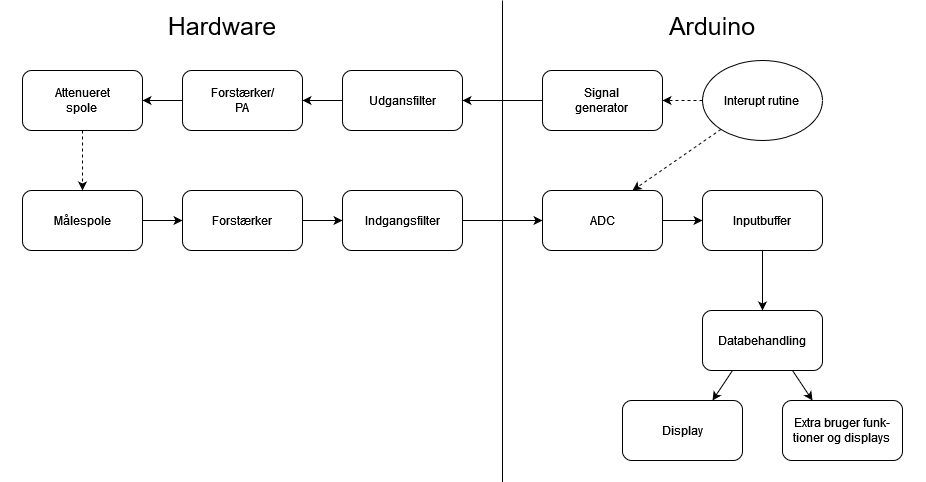
\includegraphics[width=\textwidth]{Overleaf/Pictures/Diagrammer/Overordnet projektdiagram 1.png}
     \caption{Principdiagram / blokdiagram}
     \label{fig: Principdiagram/blokdiagram}
     \end{figure}

\subsection{Hardware}
Metaldetektoren tænkes implementeret todelt med hhv. en hardware-del, bestående af diskrete komponenter, samt en mikrocontroller-del som realiseres med opsætning og kodning af en arduino.\par
Hardwaredelen tænkes implementeret i flere stadier. Først tænkes et fra arduinoen sendt signal forstærket og moduleret for at klargøre dette til at blive sendt i gennem transmitterspolen (TX).
En modtagerspole (RX) vil opfange et retursignal (RX-signal) med information omkring tilstedeværelsen af metal i metaldetektorens søgeområde, samt dennes egenskaber/type.
RX-signalet vil herefter blive forstærket og filtreret så et så vidt muligt støjfrit signal, tilpasset arduinoens måleevner, gøres klar til sampling af arduinoens ADC-modul.
\newpage
\subsection{Arduino}
Arduinoen tænkes implementeret til at skabe den oprindelige form af TX-signalet, at måle og digitalisere RX-signalet og udfører databehandling på, samt displaye, det målte RX-signal.
En tilstandsmaskine ønskes at anvendes til kontrol og styring af de forskellige funktioner.

\subsubsection{I/O signaler}
Da fasedrejningen af det målte RX-signal ønskes at anvendes til at bestemme det målte metals type er det nødvendigt at synkronisere målingen af RX-signalet med udsendelsen af TX-signalet fra arduinoen. Dette ønsker vi at implementere ved at styre udgangsfunktionsgeneratordelen og ADC'ens start-trigger gennem den samme timer, og herunder samme service rutine (ISR).

\subsubsection{Databehandling og display}
Den målte data ønskes behandlet med en variation af DFT (diskret-tids fourier transformation) for at finde signalets amplitude og fasedrejning. Ud fra dette ønskes at kunne fremvise disse værdier, samt eventuelle konklusioner baseret på data, som f.eks. det målte metals type/egenskaber.

\section{Styring af kraftværk}
Kraftværket skal styres så der altid leveres 15V til indgangen på Buck Converteren. Da belastningerne kan ændre sig, er det ikke nok blot at sætte en proportional gain på. Der er nødt til at designes et system med feedback, så den aktuelle spænding kan sammenlignes med den ønskede. Dette realiseres med en PI-Lead kontroller, der udarbejdes efter de metoder vi lærte i kurset \emph{34722 - Reguleringsteknik 1}.

Første skridt var at modellere systemets egenskaber i Matlab. Dette blev gjort ved at lave små steps på inputtet (PWM Duty Cycle) og måle hvordan outputtet reagerer. Derefter kan Matlab fitte en overføringsfunktion. Dette kan ses i nedenstående graf, hvor den grå linje er det reelle output (ADC værdier) og G er den fittet overføringsfunktion.

\begin{figure}[H]
      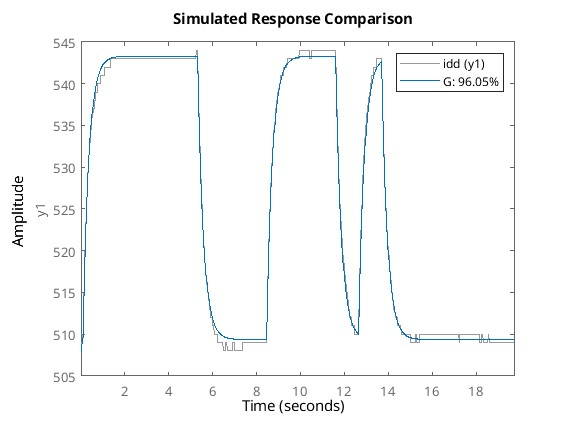
\includegraphics[width=\textwidth]{Dokumentation/Motor Model Fit.jpg}
     \caption{System Overføringsfunktion}
     \label{fig: System Overføringsfunktion}
     \end{figure}

Derefter kan PID kontrolleren nu designes. Vi vælger en phase margin på 60 grader, da det giver en god balance mellem hastighed og stabilitet. Vi tilpasser Ni og alpha værdierne indtil vi finder et system der hurtigt, men ikke så hurtigt at motoren ikke kan følge med. Nedenstående figur viser en step respons af systemet med PID kontroller. Der er en smule overshoot, men det gav ikke nogle stabilitetsproblemer.

Nu skal denne PID kontroller, som er en overføringsfunktion i S-domænet, omdannes så den kan blive implementeret i kode. Dette gøres ved at Z transformere den med en indbygget Matlab funktion, hvor vi bruger ADC samplingsraten som input. Transformationens parametre skrives til en Data.h fil, som resten af C-koden benytter. Dette gør at vi kan iterere hurtigt og præcist. Z transformationens parametre kan nemt implementeres ved at gemme forrige inputs og outputs, og gange dem med et specifikt gain. I vores tilfælde gemmes der 2 forrige outputs og 1 forrigt input. Derefter ganges hvert input/output med deres tilhørende parameterværdi og alle værdierne lægges sammen. Dette outputtes som 

     
\end{document}